\documentclass[runningheads,a4paper]{llncs}

\usepackage[utf8]{inputenc}
\usepackage{graphicx}
\usepackage{listings, color}
\usepackage[bookmarks,bookmarksopen,bookmarksdepth=2]{hyperref}


\graphicspath{ {./img/} }

\begin{document}

%============================================================

\title{A Comparison of\\ Traceability in MDE Mega-Models}
\author{Maximilian Meffert}
\institute{University of Koblenz-Landau}
\maketitle

%============================================================

\begin{abstract}

Traceability and mega-modeling deliver a strong foundation to comprehend and work with big systems.
But the research on traceability has not yet reached a common agreement nor has it reached standardization.
Although especially MDE could benefit from a strong support of traceability for the engineering of new or the analysis of existing enterprise systems.
This paper gives an overview of the current state of traceability and its support in selected MDE mega-models.


\keywords{
traceability,
mega-models,
requirement engineering,
model driven engineering,
architecture frameworks
}


\end{abstract}

%============================================================

\section{Introduction}\label{sec:Introduction}
Software and computer systems tend to become bigger and more complex to meet higher expectations.
At the same time the complexity of engineering processes creating and maintaining such systems increases proportionally.
One way of taming this rising complexity is the concept of traceability, which can be interpreted as the ability \textit{''[...] to describe and follow the life of software artifacts [...]''} \cite{ScopedTraceability}.
However, the research on traceability has not yet reached a common agreement nor has it reached standardization.

Other means to describe such big systems are mega-models, due to their high level of abstraction.
Mega-models are commonly understood as models, which use other models as their elements.
These models can be used to study technological spaces \cite{MEGAL1}\cite{MEGAL2}\cite{TowardsAMegamodel} or to provide the core for modeling tools \cite{MEGAF}\cite{DHMM}, such as used in the Model Driven Engineering (MDE) world. 
Especially the latter might benefit from the support of traceability during the engineering of large enterprise systems.

In this paper we will outline the basics of traceability.
That is, we will explore the several definitions of traceability given over time and introduce the nature of information traceability has to deal with.
Further, we will elaborate on how traceability can be divided in different categories and explain what kind of objectives might be achieved with sufficient traceability support.
Following that, we will deduce a comparison scheme to analyze several selected MDE mega-models regarding their support of traceability.

\subsubsection{Contributions of this paper}
These are the contributions of this paper:
\begin{itemize}

\item
We propose a simple, non-disjoint categorization of traceability objectives.

\item
We propose a simple comparison scheme to examine MDE mega-models regarding their support of traceability.
That is, the comparison regarding traceability link types, traceability categories and traceability objectives.

\item
A comparison of the following mega-models: 
 The MDE-Mega-Model \cite{TowardsAMegamodel},
 MEGAF \cite{MEGAF},
 MegaL \cite{MEGAL2},
 Dynamic Hierarchical Mega-Models \cite{DHMM}

\end{itemize}

\subsubsection{Non-Contributions of this paper}
These are non contributions of this paper:
\begin{itemize}

\item
We do not propose a new definition for traceability.

\item
We do not propose a new understanding of traces and traceability links.

\item
We do not propose a new traceability classification.

\item
We do not propose new traceability objectives.

\end{itemize}

\subsection{Road-map}
\label{ssec:Road;ap}
§\ref{sec:Traceability} introduces the concept in terms of origins, motivation, terminology and classification of traceability.
§\ref{sec:Comparison-of-MDE-Mega-Models} introduces a comparison scheme and applies it to selected MDE mega-models.
§\ref{sec:Conclusion} concludes the paper.


%============================================================

\section{Traceability}
\label{sec:Traceability}
This section introduces the concept of traceability.
It is based  on Winkler and von Pilgrim \cite{TraceabilitySurvey}, who compiled a complete survey on the subject.
At first we give a brief overview of the historical origins of traceability.
Secondly we explore several definitions of traceability given over time.
Then we explain actual means to describe traceability information by introducing traces and traceability links.
And finally we discuss the objectives of traceability.


\subsection{Traceability Origins}
\label{subsec:Traceability-Origins}
Historically the research on traceability in software engineering originates from requirement engineering (RE) \cite{TraceabilitySurvey}. 
The question is: given a discrete set of requirements, how can one validate or even prove that all requirements are met? 
And more importantly on what information can one base such validation? 

The idea to solve this problem came through observation on typical product development processes:
\begin{enumerate}

\item
A raw vision is extended to concrete set of requirements,

\item
then requirements are reworked into architecture,

\item
and finally the architecture is transformed to an implementation.

\end{enumerate}
Due to the incremental and iterative nature of such processes it seemed reasonable to assume, that engineering activities might leave traces, which reflect the performed activity and the past state of the modified artifact.

Later traceability became of more interest to the MDE community. 
The purpose of traceability here did not much differ from its purpose in requirement engineering. 
We just change our perspective on how we see and describe engineering processes. 
Usually we try to regard artifacts as models of some kind, at best specified by meta-models.
Activities are seen as also well defined model-transformations. 
On top of that MDE is strongly interested in the automation of engineering processes.


\subsection{Traceability Definitions}
\label{subsec:Traceability-Definitions}
Traceability is subject of various research fields, hence there is no commonly agreed definition on what traceability actually is. 
In the following text we will discuss several definitions given over time.

\begin{definition}
\label{sec:Traceability-LagoEtAl}
\textit{''Traceability is the ability to describe and follow the life of a software artifact and a means for modeling the relations between software artifacts in an explicit way.''} \cite{TraceabilitySurvey}
\end{definition}
Traceability definition \ref{sec:Traceability-LagoEtAl} is given by Lago et al. \cite{ScopedTraceability}.
This definition is where the introductory citation is taken from.
It is a good starting point if one wants to grasp what traceability is about, because it is based on the life-cycle of artifacts and their relationships, which has a nice intuitive notion. 
However, there is a weakness. 
It is not clear whose ability it should be.
It could be the ability of an engineer, as traceability is also stated to be \textit{''a means for modeling''}. 
But that would rather make it part of a personal skill set than an inherent aspect of software projects.


\begin{definition}
\label{def:Traceability-GotelFinkelstein}
\textit{''The ability to describe and follow the life of a requirement in both a forwards and backwards direction (i.e. from it origins, through its development and specification to its subsequent deployment and use, and through periods of on-going refinement in any of these phases).''} \cite{TraceabilitySurvey}
\end{definition}
Traceability definition \ref{def:Traceability-GotelFinkelstein} is given by Gotel and Finkelstein \cite{GotelFinkelstein}.
It originates from RE research, as the subject of traceability is \textit{''the live of a requirement''}.
But it facilitates a broader view by exemplifying the life-cycle of requirements throughout a software project. 
That is by implicitly extending the definition to traceability for all artifacts, because most artifacts are deployed and used according to requirements \cite{TraceabilitySurvey}.


\begin{definition}
\label{def:Traceability-PaigeEtAl}
\textit{''[...] the ability to chronologically interrelate uniquely identifiable entities in an a way that matters. [...] [It] refers to the capability for tracing artifacts along a set of chained [manual or automated] operations.''} \cite{TraceabilitySurvey}
\end{definition}
Traceability definition \ref{def:Traceability-PaigeEtAl} is given by Paige et al. \cite{PaigeEtAl}.
It is expanded on all artifacts, which can exists during the a software development process.
Also, it is stated that traceability creates a chronological order for the artifacts, following the applied operations.
Winkler and von Pilgrim emphasized the fact, that these operations could either be manual or automated.
For example a developer could have programmed a snipped of code himself, or he could have generated it.
However, the definition is somewhat ambiguous, as artifacts are interrelated \textit{''in a way that matters''}.
This could be a weakness or a strength of this definition.
In any case, it gives engineers the freedom to use traceability suitable to their needs.


\begin{definition}
\label{def:Traceability-IEEE-1}
\textit{''The degree to which a relationship can be established between two or more products of the development process, especially products having a predecessor-successor or master-subordinate relationship to one another.''} \cite{IEEEGlossary}.
\end{definition}
Traceability definition \ref{def:Traceability-IEEE-1} is the first one given by the IEEE \cite{IEEEGlossary}.
Here, traceability is not seen as an ambiguous ability.
On the contrary, it is stated as a degree of historical or hierarchical relationships. 
The notion of degree expresses the hope, that traceability is a metric between software artifacts.


\begin{definition}
\label{def:Traceability-IEEE-2}
\textit{''The degree to which each element in a software development products establishes its reason for existing.''} \cite{IEEEGlossary}.
\end{definition}
Traceability definition \ref{def:Traceability-IEEE-2} is the second one given by the IEEE \cite{IEEEGlossary}.
It still emphasizes the fact, that traceability should be a measurable degree, not someones ability.
Moreover in this definition product elements are made accountable for their own traceability.
They are bound to justify their existence, which can include naming the relationships between them and their predecessors or masters, or vice versa.


This is a unsatisfactory starting position for further elaboration.
So far, we presented five differing definitions, but there are more we have omitted.
Some differences can be explained by their different research origins.
However, those differences do not seem to be the relevant ones, as traceability of a requirement can easily extended to a general artifact traceability.

On the other hand, one difference which seems to matter is the one between the notions of ability and degree.
The usage of the former is mostly ambiguous in terms of ownership.
It is not clear if it is the ability of an engineer, a tool or of the artifact itself.
The usage of the latter expresses the desire for traceability to be a metric, inherently there, only depending on measurement.

For this report, we do not propose a new definition. 
However, we encourage to understand traceability as the ability to make use of \textit{traceability information} (traces).
Therefore, it is not important who or what the carrier of the ability is.
It can be there or not.
But traceability information should exist in every development environment for every project.
The nature of such information will be explored in the following sections.

\subsection{Traceability Information}
\label{subsec:Traceability-Information}
The second question, which motivated research on the subject of traceability was:
On what information could one base requirement coverage?
The vital idea to answer this question was the observation, any engineering activity leaves a trace.
A very simple trace would be the outcome of a \texttt{diff} in a version control system, which shows the changes of an artifact between two revisions.
However, traces can be more complex, if we consider the contents of the change. 
Source-Code could contain documenting comments, explaining what has changed and more importantly why.
The following text will introduce the basic terminology and means for describing such traceability information.


\subsubsection{Traces}
\label{subsubsec:Traces}
The most basic form of traceability information is called a \textit{trace}. 
Such traces may appear in form of meta-information, describing hard facts like \textbf{what} happened, \textbf{who} did something or \textbf{when} it happened. 
I.e. most common file systems record the owner, modification date and the last access date of a file.

Opposing that, traces also may appear as \textit{''... (non-) material indication or evidence ...''} \cite{OED} on \textbf{why} or \textbf{how} something happened. 
For example version control systems automatically record the user, modification date and the modification itself committed for a given artifact.
Additionally a commit-message is passed alongside which hopefully gives some insights on the stored changes.
These messages could refer to a customer interview, a discussion under colleagues or technical research to establish some reason on the modification\footnotemark.
Such conversations are usually not transcribed, hence they are considered soft traceability information.

\footnotetext{Note, the modification itself is also considered to reflect such non-material traceability information. 
Although this data is hard to obtain unless there is explicit documentation like sufficient comments or commit-messages.}

Following this separation in hard and soft fact traces, Pinheiro \cite{Pinheiro} defines a classification which somewhat resembles the separation commonly used on requirements:
\begin{itemize}

\item
\textbf{Functional traces:}
Traces existing due to well defined transformations. 
Such transformations produce traces as by-products like revision numbers in version control systems. 
Or traces that may be obtained by analyzing the transformation input, output and rules. 
In short, these traces have to obey some sort of formalism.

\item
\textbf{Non-Functional traces:}
Traces which cover \textit{''reason, context, decision, and technical''} \cite{TraceabilitySurvey} aspects. 
I.e. explaining correction due to edge case testing.

\end{itemize}

\subsubsection{Traceability Links}
\label{subsubsec:Traceability-Links}
One IEEE definition of a trace is:
\textit{''[...] a relationship between two or more products of the development process;
for example, to establish the relationship between a given requirement and the design element that implements that requirement.''} \cite{IEEEGlossary}. 
The notion of relationships describing or supporting traceability leads to the concept of \textit{traceability links}.
These links can be seen as a special case of traces.
They are stated to be instances of n-ary, multi-directional relations. 
However, the direction of a traceability link does not limit the navigation direction. 
Links can always be navigated in both forward and backward direction.

\begin{figure}
\centering
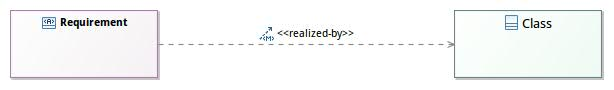
\includegraphics[width=\textwidth]{SimpleRealizationTraceabilityLink.jpg}
\caption{Requirement realization link}
\label{fig:RequirementRealizationLink}
\end{figure}

The IEEE example for traceability links is shown in Figure \ref{fig:RequirementRealizationLink}, where the unidirectional realization link of a requirement by a class is denoted. 
Although, unlike traces, traceability links are not explicitly named by the IEEE Glossary.
Therefore they are often used as synonyms for one another \cite{TraceabilitySurvey}.
Figure \ref{fig:RequirementRealizationLink} is a minimal example, in real-life the relation might need a higher arity to add constrains and test cases in order to confirm realization.
The relation between two versions of an artifact in the revision history or the Parent-Child relation between classes would be other examples of such traces.


\subsubsection{Traceability Link Types}
\label{subsubsec:Traceability-Link-Types}
Many researchers suggested that traceability links should be classified in types, depending on the relationship they are depicting \cite{TraceabilitySurvey}.
Given the example shown in Figure \ref{fig:RequirementRealizationLink}, a suitable type for this link could be \textit{Requirement Realization}.
But, this would be a type for only one case.
The suggested types usually share a higher granularity.

Aizenbud-Reshef et al.\cite{Aizenbud-Reshef} included a simple classification in their definition for traceability links.
Although the proposed class were meant to be actual types, they can be read as such. 
It contains: 
 explicit links or as a result of transformations (code generation or reverse engineering),
 computed links  based on existing information (code dependency analysis),
 statistically inferred links based on history by a revision systems \cite{TraceabilitySurvey}.
Spanoudakis and Zisman \cite{SpanoudakisAndZisman} created a more complex type system from literature:
\begin{itemize}

\item
\textbf{Dependency Links}
denoting that changes in the depended artifact may result in changes in the depending artifact

\item
\textbf{Refinement Links}
denoting abstraction or composition hierarchies between artifacts.

\item
\textbf{Evolution Links}
denoting an Argument-Result relation between artifacts, the transformation of one artifact into an other

\item
\textbf{Satisfiability Links}
denoting compliance of a lower artifact with a higher one

\item
\textbf{Overlap Links}
denoting that artifacts share information, but differ in representation

\item
\textbf{Conflict Links}
denoting that a there exists a conflict between artifacts

\item
\textbf{Rationalization Links}
denoting the justification for the creation or evolution of artifacts

\item
\textbf{Contribution Links}
denoting that a stakeholders shares interests with certain artifacts

\end{itemize}

Moreover, given the fact that traceability links can be seen as special cases of traces, the high order classification in Functional and Non-Functional could also be regarded as types.




\subsection{Traceability Categorization}
\label{subsec:Traceability-Link-Categorization:}
Similar to the several different definitions and type systems of traceability and traceability links, there is also no commonly agreed categorization system for traceability in general.
However, most categorizations seem consider the phase or refinement nature of the traceability information.

In RE research, there is the distinction between \textit{pre- and post- requirement specification traceability} by Gotel and Finkelstein \cite{GotelFinkelstein}.
These categories divide the development process in the two big phases before and after the specification of requirements.
In contrast to that, Ramesh and Edwards \cite{RameshEdwards} make a distinction between whether an artifact is traceable across refinement layers or not.
This is called \textit{horizontal and vertical traceability}.
Figure \ref{fig:RequirementRealizationLink} exemplifies vertical traceability, because realization is a relation between refinement layers.
Horizontal traceability could exist alongside a class dependency (e.g. Dependency Injection).

Additionally, there are also categorizations originating from MDE research. 
Paige et al. \cite{PaigeEtAl} also propose a big phase categorization system alongside the life-cycle of models:
\begin{itemize}

\item
\textbf{Pre Model Traceability}
considers traceability between the first non-model artifacts and the first models

\item
\textbf{Intra Model Traceability}
considers traceability between models during model-refinement

\item
\textbf{Post Model Traceability}
considers traceability between the final model and artifacts generated by that model

\end{itemize}


\subsection{Traceability Objectives}
\label{subsec:Traceability-Objectives}
Finally we want to further elaborate the benefits of traceability.
The initial motivation behind the subject was the validation of requirement coverage.
But general artifact or model traceability can achieve more than that.

\begin{figure}
\centering
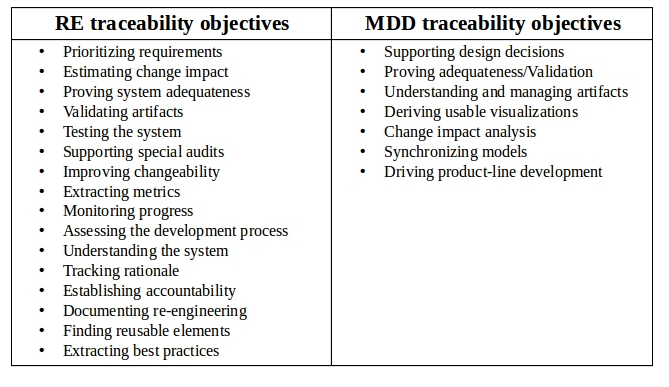
\includegraphics[width=\textwidth]{TraceabilityObjectives.jpg}
\caption{Traceability Objectives identified by Winkler and von Pilgrim \cite{TraceabilitySurvey}}
\label{fig:TraceabilityObjectives}
\end{figure}

Winkler and von Pilgrim \cite{TraceabilitySurvey} identified several objectives, where traceability might be of great help. 
Figure \ref{fig:TraceabilityObjectives} depicts traceability objectives sorted by the research field they originated from. 
However, most objectives found in requirements engineering can also be considered important to the MDE community. 
Additionally some objectives already correspond directly.
For example \textit{Estimating change impact} and \textit{Change impact analysis} do not differ at all regarding their purpose. 
Given sufficient traceability information in form of traces and traceability links, one can simulate changes top-down to the final model and estimate their impact on metrics like quality, performance, and cost. 
The only difference between RE and MDE here lies in the propagation of changes. 
Where in RE changes are considered to be propagated manually, MDE uses automation. 
Although nowadays RE also relies on tool support.

Other corresponding objectives are \textit{Proving system adequateness}/\textit{Validating artifacts} and \textit{Proving adequateness/Validation}. 
If end-to-end traceability from early artifacts to the final implementation is achieved, one cannot only use traces to identify incompleteness (top-down), it is also possible to check for requirement coverage (bottom-up).
This is especially beneficial for the use case to attest customers that the system specification is met and not exceeded.

Besides these product centric objectives, which mainly address maintainability and soundness concerns of a completed project, there are also objectives, which support the development process itself.
Such are \textit{Monitoring progress} and \textit{Establishing accountability}, where project management can leverage end-to-end traceability to determine if a milestone is reached, or who to blame if not. 
Eventually we can learn from collected traceability data during a project revision while \textit{Extract Best Practices} to support future design decisions. 

All these objectives can be further categorized regarding stakeholders or general purpose.
We propose the following categorization:
\begin{itemize}

\item
\textbf{Technical Comprehension}
considers objectives regarding the technical understanding of the system.
The interests here lie in the supporting the actual engineering activities.
(Supporting special audits,
Improving changeability,
Proving system adequateness,
Extracting metrics,
Tracking rationale,
Finding reusable elements,
Documenting re-engineering, 
Supporting design decisions,
Change impact analysis,
Synchronizing models,
Extracting best practices,
Understanding the system,
Extracting best practices)


\item
\textbf{System Management}
considers objectives regarding management decisions. 
It is not concerned with technical details.
The interests here lie in the monitoring of progress and accountability.
Additionally, we are interested in the extraction of knowledge to support future decisions.
(Prioritizing requirements,
Proving system adequateness,
Extracting metrics,
Monitoring progress, 
Assessing the development process,
Establishing accountability,
Documenting re-engineering,
Extracting best practices,
Change impact analysis,
Driving product-line development,
Understanding the system)

\end{itemize}
However, those categories are not disjoint.
That is because both fields do not exist in isolation.
Management needs at least some general understanding of the system.
On the other hand, technical decisions must also consider some management aspects.
And eventually, a single achieved objective is beneficial for both fields.
For instance, consider \textit{Change impact analysis}:
In the sense of Technical Comprehension, traceability can provide all entities, that also might need to be changed.
In the sense of System Management, traceability can support estimating time and cost of the changes. 

%============================================================

\section{Comparison of MDE Mega-Models}
\label{sec:Comparison-of-MDE-Mega-Models}
One main goal of this paper is to provide a comparison of contemporary MDE Mega-Models regarding their support of traceability.
The term mega-model is somewhat ambiguous as it commonly refers to models using other models as their elements. 
But the term model is not used in a restrictive manner \cite{MEGAL2}.
It can be interpreted as intuitive models, elements of such models, meta-models describing such models, and moreover the term may be used for mega-models itself.
So mega-models could actually describe mega-mega-models or even mega*-models. 

Mega-models are valuable to MDE, because they can be used for large-scale modeling, i.e. models of big enterprise systems \cite{TowardsAMegamodel}. 
Such systems are ecosystem-like environments consisting of various different technologies interacting with each other. 
Especially regarding this aspect of systems, one can make use of mega-models to investigate the dependencies of involved \textit{technological spaces} \cite{MEGAL1}\cite{MEGAL2}\cite{TowardsAMegamodel}. 
However, the use of mega-models may not only be indicated by system size. 
Even minimal static (in a sense that content is not provided dynamically, e.g. by databases) web-pages can use a multitude of technologies in form of:
\begin{itemize}
\item software languages like HTML, CSS and JavaScript (nowadays CSS also may conform to corresponding LESS or SASS code),
\item software APIs likes JQuery, Angular.js, etc.,
\item infrastructure components like server and client/browser, 
\item and protocols like HTTP(S) or FTP.
\end{itemize}
Enhancing the web-page with server side logic might add the technological spaces of PHP-ware, Java-ware and/or SQL-ware.

Mega-models are also the hearts of MDE supporting tools.
MDE tools provide functionalities to create and maintain digital representations of models, meta-models and model-transformations and the dependencies between them. 
Because over time the term traceability expanded from the tracing of requirements to general artifact/model traceability, we are interested to what extend it can be covered with such models.
That is, what form of traceability information can be or is recorded by them.

In this section we first introduce the comparison scheme to compare the traceability aspects of the studied models.
Then we will apply this scheme to 
	the \textit{MDE Mega-Model}  by Favre et al. \cite{TowardsAMegamodel},
	\textit{MEGAF} by Hillard et al. \cite{MEGAF},
	\textit{MegaL} by Lämmel and Varanovich \cite{MEGAL2}
	and finally \textit{Dynamich Hierarchical Mega-Models} by Seibel et al. \cite{DHMM}.



\subsection{Comparison Scheme}
In Section §\ref{sec:Traceability} we have introduced the basics of traceability.
Because there is yet no definition that is commonly agreed upon, we do not use any definition given in §\ref{subsec:Traceability-Definitions} as distinguishing characteristic.
However, we consider traceability information to be inherently existing.
Therefore we investigate the nature of the traces, which are defined or can be excerpted.
But we do not use the broad classification of Functional and Non-Function traces given by Pinhero et al.

Mega-models and models in general are used to interrelate their entities.
Thus, following the leading notion of relationships, we consider traceability links as the main subjects of interest.
We will use the types by Spanoudakis and Zisman introduced in §\ref{subsec:Traceability-Information} to describe the meaning of identified links.

Further we try to coordinate the models within the categories by Paige et al. introduces in §\ref{subsec:Traceability-Link-Categorization:}.
And finally we use our categorization of traceability objectives introduced in §\ref{subsec:Traceability-Objectives} to describe the general intention of the identified traceability.

\subsection{The MDE-Mega-Model}\label{subsec:TheMDEMegaModel}
The MDE-Mega-Model (Figure \ref{fig:TheMDEMegaModel}) by Favre et al. \cite{TowardsAMegamodel} is an approach, that aims to model typical MDE processes and relations. 
Although it is not yet complete, it already proves to be a powerful help for analyzing technological spaces. 
\begin{figure}
\centering
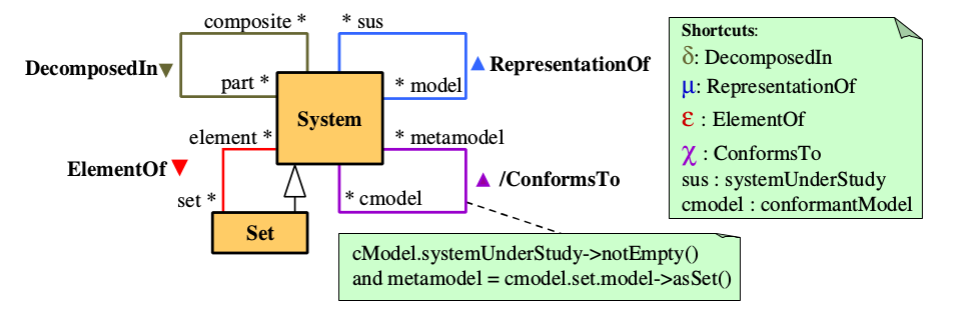
\includegraphics[width=\textwidth]{MDE-MegaModel.png}
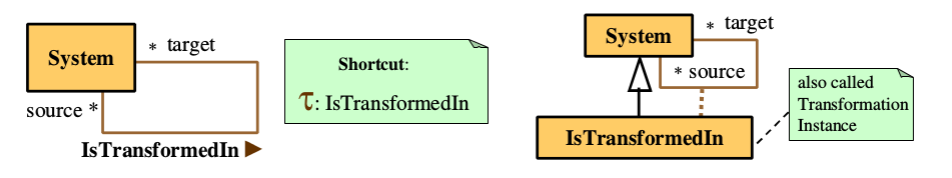
\includegraphics[width=\textwidth]{MDE-MegaModel-Transformations.png}
\caption{The MDE-Mega-Model by Favre et al. \cite{TowardsAMegamodel}}
\label{fig:TheMDEMegaModel}
\end{figure}
Favre et al. identify five relations concerning systems which we will now explain in short:

\textbf{systems}
At first we need to clarify the term \textit{system}. 
Favre et al. state: \textit{''A system is the primary element of discourse when talking about MDE''}.
Although, the usage of this term is not important, as everything can be seen as some kind of system \cite{TowardsAMegamodel}. 
This is exemplified with the trigonometric system $\pi$ (meaning the real number). 
For the sake of simplicity and not repeating examples we may just think of a system as the \textit{entity of interest}.

\textbf{$\delta$ (\texttt{DecomposedIn})}
Decomposition is a structural relationship which denotes that a \textit{composite} can be \texttt{DecomposedIn} a \textit{part}, or in set-theoretic notation: 
\begin{center}
\textit{composite} $\delta$ \textit{part} or $(composite, part) \in \delta$
\end{center}
Example: 
A directory in a file system tree contains simple files and other directories, so its safe to say: 
\texttt{dir} $\delta$ \texttt{file} and \texttt{dir} $\delta$ \texttt{dir}. 
The latter also illustrates the recursive notion of this relation.

\textbf{$\mu$ (\texttt{RepresentationOf})}
Representation is a descriptive relationship denoting a \textit{model} as a \texttt{RepresentationOf} of a \textit{system under study}. 
We write:
\begin{center}
\textit{model} $\mu$ \textit{sus}
or 
(\textit{model},\textit{sus}) $\in\mu$
\end{center}
Again, we do not care that much about the term \textit{system}, for \textit{model} on the other hand we think of it as abstraction and/or simplification of such systems.
Example: 
Directories contain $n$ files, a list of files can be the representation of a directory: \texttt{[file0,file1,...]} $\mu$ \texttt{dir}.

\textbf{$\varepsilon$ (\texttt{ElementOf})}
This is simply the set-theoretic $\in$ relationship, so an \textit{element} is \texttt{ElementOf} a \textit{set}. In greek notation:
\begin{center}
\textit{element} $\varepsilon$ \textit{set}
or 
(\textit{element},\textit{set}) $\in\varepsilon$
\end{center}
Example: 
\texttt{FOO := (/foo)+} is the set of all Unix-files following the this pattern ( \texttt{FOO = \{ /foo, /foo/foo, /foo/foo/foo, ... \} } ).
So \texttt{/foo} $\varepsilon$ \texttt{FOO}.

\textbf{$\chi$ (\texttt{ConformsTo})}
Conformance adds the notion of meta-models, where a \textit{conformantModel} \texttt{ConformsTo} a \textit{metamodel}.
\begin{center}
\textit{cmodel} $\chi$ \textit{metamodel}
or 
(\textit{cmodel},\textit{metamodel}) $\in\chi$
\end{center}
Example: 
\texttt{(/foo)+} is a model for \texttt{FOO}, \texttt{/foo(/foo)*} is also one, so we have \texttt{(/foo)+} $\mu$ \texttt{FOO}. 
Both are regular expressions describing the same set of strings and thus have to obey the syntax rules for regular expressions (\texttt{RegExp}).
Or in the notation of this mega-model: \texttt{(/foo)+} $\chi$ \texttt{RegExp}.

\textbf{$\tau$ (\texttt{IsTransformedIn})}
Transformations play a very important role in MDE because the benefit of just being able to statically describe systems is limited.
Additionally we need the ability to model the progress of a development process. 
But this is relatively simple to achieve by applying the well known concept of functions to this mega-model. 
So we may say a \textit{source} \texttt{IsTransformedIn} a \textit{target}, we think \textit{source} $\mapsto$ \textit{target} and write:
\begin{center} 
\textit{source} $\tau$ \textit{target}
or 
(\textit{source},\textit{target}) $\in\tau$
\end{center}
Example:
One transformation class of particular interest are model transformations. 
Given the established model \texttt{(/foo)+}, we might have it transformed to the model \texttt{(/bar)+}. 
This is denoted by \texttt{(/foo)+} $\tau$ \texttt{(/bar)+} or (\texttt{(/foo)+}, \texttt{(/bar)+}). 
The latter is also called \textit{transformation instance/application}.

The MDE-Mega-Model and the important role of transformations and \textit{transformation systems} can be explored in more detail in the paper by Favre et al. \cite{TowardsAMegamodel}. 
It also offers some insights on the correlation of (formal) languages and models, which enables a higher point of view on software in general. 
However, for this paper and its discussion of traceability the short introduction above is sufficient.

\subsubsection{Traceability Links}
There are five relations defined in the MDE-Mega-Model and all these links carry traceability information.
The most simple ones are $\delta$ and $\varepsilon$, both are \textbf{Refinement Links}.
Refinement Links denote hierarchies of abstraction or dependencies of aggregation and composition.
The $\delta$ relationship exactly does the latter. 
It states that a composite can be broken down into a smaller part.
In this regard, the $\varepsilon$ shares that characteristic for aggregation.
But it can also be interpreted as abstraction.

Other simple relations for comparison are $\chi$ and $\tau$.
$\chi$ defines conformance in the sense of meta-modeling.
This is a \textbf{Satisfiability Link}, which denotes upstream compliance.
However, $\chi$ is also a \textbf{Dependency Link}.
That is because changes in a meta-model can result in necessary changes on downstream entities to preserve conformance.
In that regard the traceability link types by Spanoudakis and Zisman are not exclusive. 
$\tau$ is an \textbf{Evolution Link}, which is defined to capture that one entity is transformed into another.
This could be just simple content modification, where the evolution would correspond to versioning, or it could be the generation of a parser.

The last relationship of the MDE-Mega-Model is $\mu$.
This can be an \textbf{Overlap Link} in combination with $\tau$, but this traceability link is not explicitly in the model.
Consider two transformations \texttt{toXml} and \texttt{toJson} which transform an artifact to XML or JSON:
\begin{center}
$a$ \texttt{toXml} $a_{xml}$, $a$ \texttt{toJson} $a_{json}$
\end{center}
In the notion of the MDE-Mega-Model $a_{xml} \mu a$ and $a_{json} \mu a$ would hold, so $a_{xml}$ and $a_{json}$ would be connected via an Overlap Link.

\subsubsection{Traceability Categories}
The MDE-Mega-Model is a theoretical approach to study MDE as a whole.
Hence, it cannot be clearly be categorized in one of the three categories \textbf{Pre Model}, \textbf{Intra Model} or \textbf{Post Model}.
It rather can be used in all of these phases of the MDE process.

\subsubsection{Traceability Objectives}
As stated before, the MDE-Mega-Model as a theoretical approach on MDE.
Its primary use case is academic research on MDE relations and dependencies \cite{TowardsAMegamodel}.
Thus major objective category that can be targeted with this model is \textbf{Technical Comprehension}.
However, since both categories are not fully disjoint, it is also possible to achieve objectives in the System Management category.
We only consider the intended use.


\subsection{MEGAF}\label{subsec:ArchitectureFrameworkMegaModels}
MEGAF\footnote{\url{http://megaf.di.univaq.it}} is an approach on global model management by Hillard et al. \cite{MEGAF} utilizing mega-models to create reusable definitions of architecture frameworks.

\begin{figure}
\centering
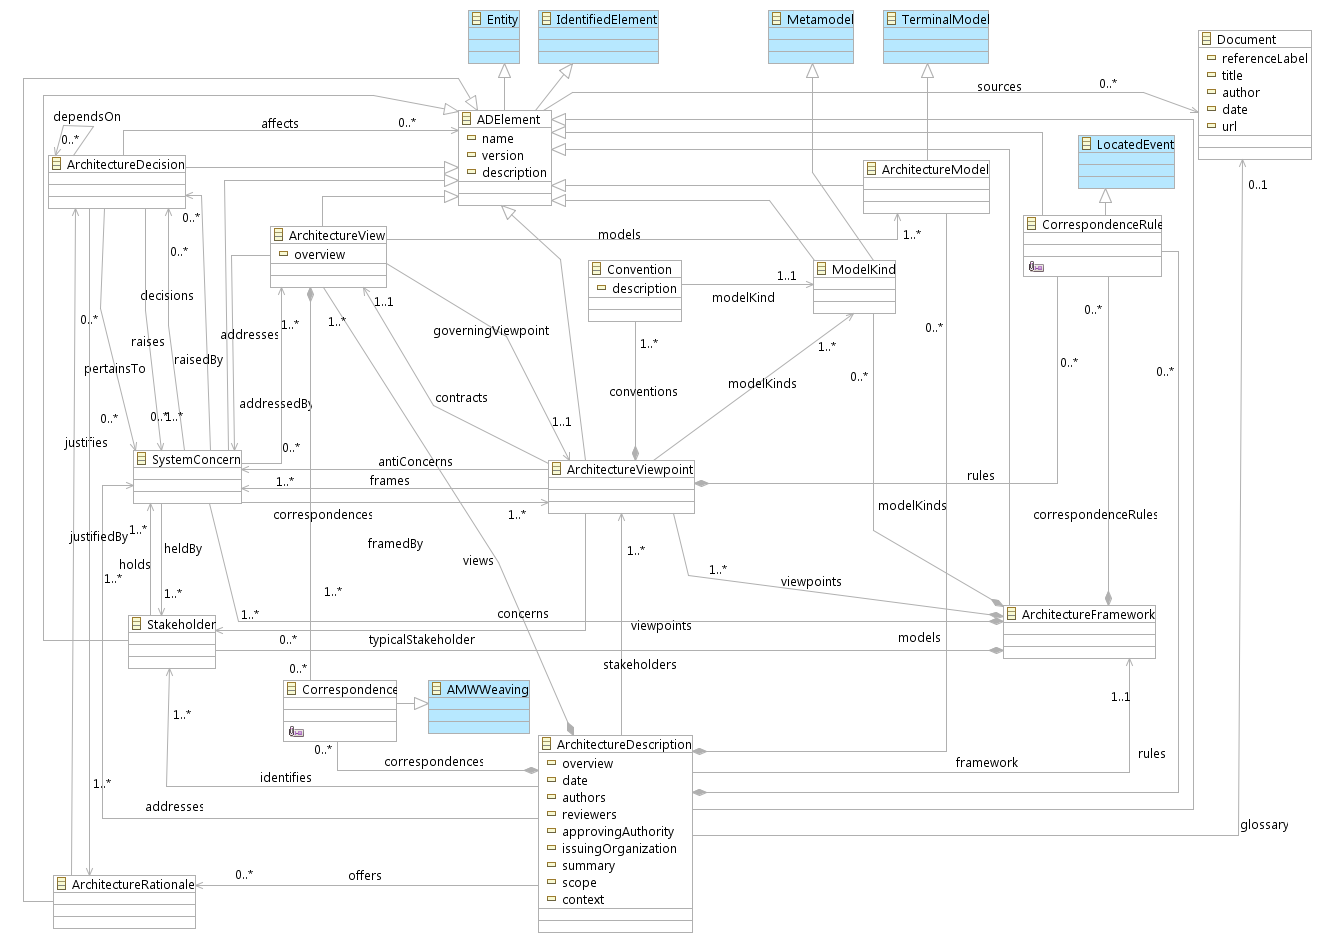
\includegraphics[width=\textwidth]{GMM4SA.png}
\caption{The GMM4SA meta-model}
\label{figure:GMM4SA}
\end{figure}

Architecture frameworks are defined by the \textit{ISO/IEC 42010 Software and System Engineering – Architecture Description} Standard \cite{ISO/IEC42010}. 
They are collections of coordinated viewpoints, conventions, principles and practices to create architecture descriptions for specific stakeholders. 
Where architecture viewpoints are collections of conventions, notations and modeling practices used to create concrete views, which address domain specific system concerns for a distinct set of stakeholders.
Their purpose is to capture and formalize a certain perspective.

According to the creators of MEGAF such architecture descriptions or frameworks alone have proven to be difficult to re-use and validate (consistency check) \cite{MEGAF}. 
So in order to fix those issues, MEGAF shall provide features to: 
\begin{itemize}

\item 
\textit{store} architecture description elements (i.e. viewpoints, views, stakeholders, models, etc.), therefore making such elements reusable

\item
\textit{define correspondence relations and correspondence rules} between architecture description elements

\item
\textit{enable correctness and completeness checks} for architecture descriptions elements

\end{itemize}

To utilize mega-modeling techniques the assumption is made, that any architecture description element may conform to its meta-model. 
So a view may conform to a viewpoint, an architecture model may conform to a model kind, etc. This is straight forward and complies with the MDE world. 
The core of MEGAF is specified in \textit{Global Model Management for Software Architecture} (GMM4SA\footnote{\url{http://megaf.di.univaq.it/images/GMM4SA.png}}) meta-model shown in figure \ref{figure:GMM4SA} as UML class diagram. 

\subsubsection{Traceability Links}
The diagram can be used to study the possible traceability of MEGAF. Because it is written in UML syntax, UML semantics apply and we already can identify several traceability links known from the MDE-Mega-Model. 
For example: {\small \texttt{ArchitectureFramework} $\delta$ \texttt{ArchitectureViewpoint}} or {\small \texttt{ArchitectureViewpoint} $\varepsilon$ \texttt{ADElement}}.
These relations exist inherent in class diagrams as association/aggregation/composition ($\delta$) and generalization ($\varepsilon$). 
Therefore, and because of the size of the GMM4SA, there are many \textbf{Refinement Links} that can be found in this model.

The relation \texttt{ArchitectureViewpoints contracts ArchitectureView} denotes that views have conform to a viewpoint.
So both entities are connected via an \textbf{Satisfiability Link}, and likewise to the MDE-Mega-Model satisfiability creates a \textbf{Dependency Link} in order to preserve conformance.

But in contrast to the MDE-Mega-Model the GMM4SA contains \texttt{Stakeholders} and an \texttt{ArchitectureRationale}, which enables additional traceability capabilities.
For instance the relationship \texttt{Stakeholder holds SystemConcern} creates a \textbf{Contribution Link}.
And the relation \texttt{ArchitectureRationale justifies ArchitectureDecision} records extra background information for the development process.
Thus it creates a \textbf{Rationalization Link}, which comparable to satisfiability propagates the creation of a \textbf{Dependency Links}.
A change in the rationale could very likely result in downstream changes.


\subsubsection{Traceability Categories}
MEGAF aims to create tool support for reusable architecture frameworks. 
Architecture frameworks can be used to inspect the model at any time during development process from a higher perspective.
So, using the categorization by Paige et. al \cite{PaigeEtAl}, MEGAF enables \textbf{Pre Model}, \textbf{Intra Model} and \textbf{Post Model} traceability.


\subsubsection{Traceability Objectives}
MEGAF is an approach on global model management.
It aims to give a high level overview over a system, and records important traceability information like contribution (stakeholders) and rationalization (architecture rationale, system concerns).
Both aspects are valuable to Technical Comprehension and System Management.
However, the high abstraction of architecture frameworks is more suitable for \textbf{System Management} objectives than it is for Technical Comprehension.


\subsection{MegaL}
MegaL is an approach on system understanding mainly concerned with the linguistic architecture of the system under study \cite{MEGAL1}\cite{MEGAL2}. 
It intents to uncover its technological footprint by revealing the used technological spaces and their interrelations. 
This is called a linguistic architecture because technological spaces of great interest are programming languages and their associated products.

\begin{figure}
\centering
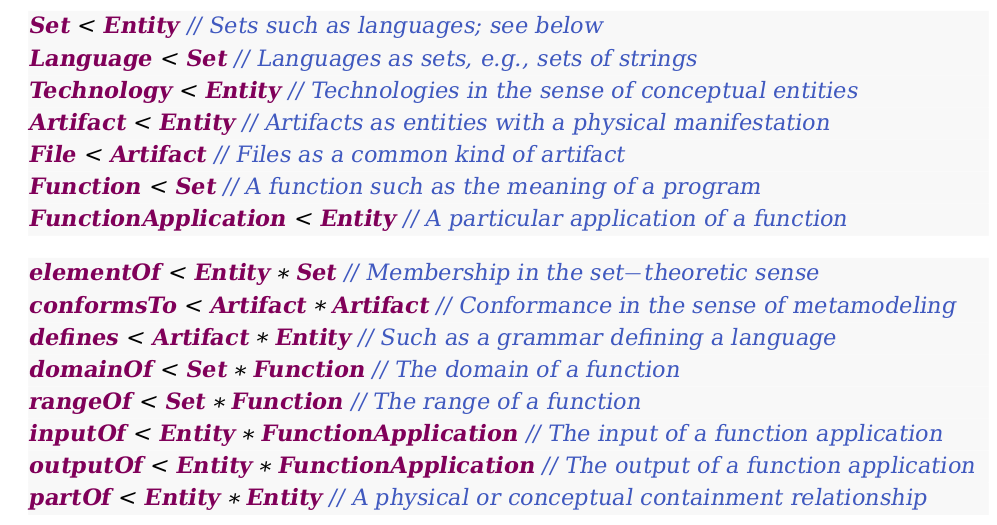
\includegraphics[width=\textwidth]{megal-definition.png}
\caption{Definition of MegaL Entities and Relationships \cite{MEGAL2}}
\label{fig:MegaL-Definition}
\end{figure}

In fact, MegaL is not only a mega-model, it is rather a mega-model description language. 
Figure \ref{fig:MegaL-Definition} shows the definition of the main entities and relationships of MegaL.
We see, it is closely related to the MDE-Mega-Model, as all relations defined there make an occurrence here too.
However, the relations of MegaL have stricter semantics.
Each relation is defined as the Cartesian product of concrete entities.

As software language, MegaL is designed to be interpreted.
Given a mega-model defined in MegaL, this mega-model can be applied to any system \cite{MEGAL2}.
To do so, Lämmel an Varanovich designed a extendable interpreter, which loads a mega-model written in MegaL and a configuration file, which contains an URI to the resource to analyze and a specification of suitable resolvers and evaluators.
Where resolvers are programs, which resolve the resource URI following Linked-Data principles (for instance a resource may be located at a distant server).
And evaluators are programs, suitable to evaluate the various MegaL relationships (e.g. the element-of-Java relation) \cite{MEGAL2}.

Unlike the models before, MegaL has build-in capabilities for \textit{traceability recovery} \cite{MEGAL2}.
Evaluators can have the ability to record traceability links as pairs of URIs:
\begin{center}
$\langle$ "http://.../MegaLParser.java/class/MegaLParser/method/megamodel/1" ,
\\"http://.../MegaL.g4/grammar/megal/rule/megamodel/1" $\rangle$
\end{center}
Here, linking the \texttt{conformsTo} relationship of class-method in the java file MegaLParser.java to the grammar rule found in the file MegaL.g4 \cite{MEGAL2}.

\begin{figure}
\centering
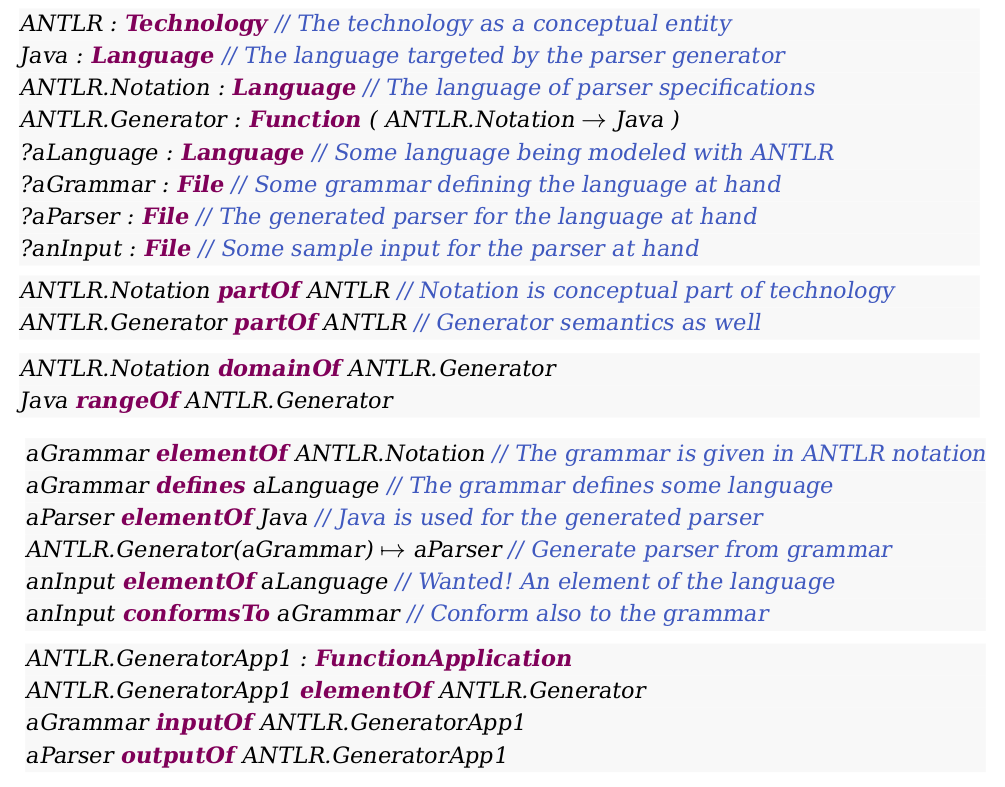
\includegraphics[width=0.7\textwidth]{megal-example-antlr.png}
\caption{MegaL Example: ANTLR Mega-Model\cite{MEGAL2}}
\label{fig:MegaL-Example}
\end{figure}

Figure \ref{fig:MegaL-Example} depicts the example usage of MegaL. 
It shows the specification of a mega-model for the ANTLR parser generator.
This example includes some shorthand notation:
\begin{itemize}

\item
\texttt{ANTLR.Notation}
(dot notation) is dissolved as part-of relationship shown in the second paragraph of Figure \ref{fig:MegaL-Example}

\item
\texttt{ANTLR.Notation $\rightarrow$ Java}
is dissolved as function definition in form domain-of and range-or relationships shown in the third paragraph of Figure \ref{fig:MegaL-Example}

\item 
\texttt{ANTLR.Generator(aGrammar) $\mapsto$ aParser}
is dissolved as function application shown in the last paragraph of Figure \ref{fig:MegaL-Example}

\end{itemize}

\subsubsection{Traceability Links}
As noted before, MegaL already has the capabilities to capture traceability links.
However, the defined captured relationships are recorded as is.
For instance the \texttt{conformsTo} relation is recored as pair of URIs.

We apply the type system of Spanoudakis and Zisman in order to compare MegaL to the other presented models.
Although, because of the great analogy to the MDE-Mega-Model by Favre et al. many traceability link types can be adopted.
That is for the relationships \texttt{elementOf}, \texttt{partOf} and \texttt{conformsTo} and \texttt{FunctionApplication} entities.
Therefore the types \textbf{Refinement Link}, \textbf{Satisfiability Link}, \textbf{Dependency Link} and \textbf{Evolution Link} including the possible \textbf{Overlap Link} exist here for the same reasons.

However, transformation here are modeled in more detail.
Functions are defined via the \texttt{domainOf} and \texttt{rangeOf}.
Thus there are also refinement links between the modeled function and other entities.
The same holds for the \texttt{inputOf} and \texttt{outputOf} relations of function applications.

\subsubsection{Traceability Categories}
MegaL is intended to analyze existing systems and technological spaces.
In that regard it can be categorized to support \textbf{Post Model} traceability.
However, like its related model, the MDE-Mega-Model, it is also meant for research purposes,
With its flexible design regarding resolver and evaluator plug-in-system, it could easily be used to analyze models from the pre and intra model phases of MDE processes.


\subsubsection{Traceability Objectives}
Lämmel and Varanovich clearly state that MegaL is especially designed for \textit{''[...] modeling the linguistic architecture of software systems, i.e., a system’s architecture in terms of relationships between conceptual entities such as languages and technologies as well as actual entities [...]''} \cite{MEGAL2}.
This is best out with the objective \textit{Understanding the system}.
Hoever, this objective is found in both categories.
But the extend, to which \textbf{Technical Comprehension} is offered by MegaL seems to exceed the level understanding needed for System Management by far.


\subsection{Dynamic Hierarchical Mega-Models}
Dynamic Hierarchical Mega-Models (DHMM) are an approach on traceability link management by Seibel et al. \cite{DHMM}.
It is meant to be used as the core of a proposed model environment.
The DHMM actually models how traceability links interrelate with entities and also models their nature regarding types.
In that aspect it differs greatly from the previously analyzed models.

\begin{figure}
\centering
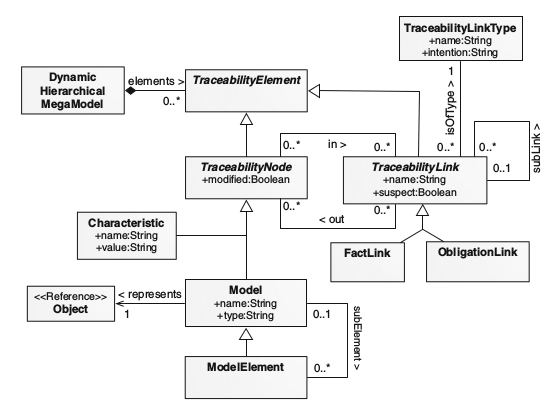
\includegraphics[width=0.5\textwidth]{dcmm.png}
\caption{Meta-Model of the Dynamic Hierarchical Mega-Model \cite{DHMM}}
\label{fig:DHMM-Meta-Model}
\end{figure}


Figure \ref{fig:DHMM-Meta-Model} depicts the relevant part of the DHMM meta-model.
It shows that a traceability link connects two traceability nodes like models or model elements.
It is also shown that a traceability link is of exactly one type and either is a FactLink or an ObligationLink.
Fact links describe simply that a modeled intention between to artifacts hold, thus they are facts \cite{DHMM}.
Obligation links describe that \textit{''the instantiation of some arbitrary operation [...] satisfy the intention [and thus the obligation] should hold''} \cite{DHMM}.
These links a meant to be placed by human modelers.
In that regard Seibel et al. seem to follow the classification of traces in Functional (fact) and Non-Functional (obligation) by Pinheiro et al. \cite{Pinheiro}.
Where the former trace have to obey some sort of formalism and the latter need to cover \textit{''reason, context, decision, and technical''}\cite{Pinheiro}.

\begin{figure}
\centering
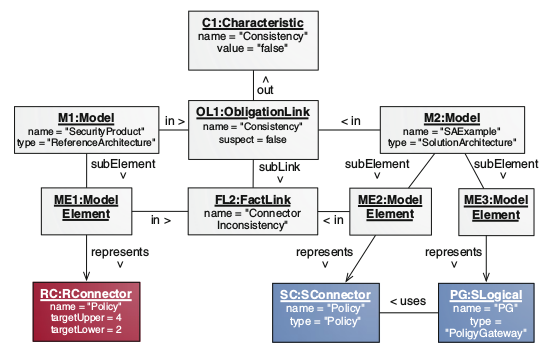
\includegraphics[width=0.5\textwidth]{dcmm-example.png}
\caption{Top-Down Hierarchy of Traceability Links \cite{DHMM}}
\label{fig:DHMM-Example}
\end{figure}

The key aspect of DHMMs is the notion hierarchy. 
In Figure \ref{fig:DHMM-Meta-Model} it is defined by the sub-link self-association.
Any traceability link can have multiple sub-links.
This is exemplified in Figure \ref{fig:DHMM-Example}, which shows a top-down hierarchy. 
A modeler has placed an obligation link between to models to ensure the consistency between them.
Figure \ref{fig:DHMM-Example} further shows, that a validation mechanism has found an inconsistency and therefore deduced a fact link between the model elements one hierarchy level beneath.
The inconsistency here lies in the fact that the RConnector policy demands at least two connections.
However, there is only one SConnector.
DHMMs can also have bottom-up hierarchies, but we omit those here.

\subsubsection{Traceability Links}
Because the DHMM is an actual traceability link management model, which includes the model for link types, we cannot identify any further types following the comparison scheme.
So, we could just conclude that custom types are allowed.
However, Figuer \ref{fig:DHMM-Example} shows the deduction of a traceability link denoting an inconsistency.
This can be classified as a \textbf{Conflict Link} according to Spanoudakis and Zisman.
Moreover, one big aspect of DHMMs is the validation of created traceability links, which can easily result in many of such Conflict Links.

\subsubsection{Traceability Categories}
The DHMM is the heart of a modeling environment proposed by Seibel et al \cite{DHMM}.
Therefore, it is meant to create and maintain models. 
That makes it fall in the \textbf{Intra Model} traceability category.
However, depending on the extend of the model managed by the DHMM, in the sense that artifacts generated by such model are also managed, it also falls in the Post Model traceability category.


\subsubsection{Traceability Objectives}
Similar to traceability categories, DHMMs are meant for tool support grade of traceability.
Traceability link types can be dynamically defined by modelers \cite{DHMM}.
Any kind of traceability information could be recorded and analyzed to provide knowledge for System Management.
However, Seibel et al. made great efforts to optimize DHMMs for validation and automation \cite{DHMM}.
The intended use is clearly stated to be for human modelers, i.e. technical staff.
So it seems the main objectives of DHMMs lie in the category of \textbf{Technical Comprehension}.


%============================================================

\section{Conclusion}\label{sec:Conclusion}
We compared the MDE-Mega-Model, MEGAF, MegaL and Dynamic Hierarchical Mega-Models regarding their support of traceability.
We used the traceability types proposed by Spanoudakis and Zisman \cite{SpanoudakisAndZisman}, the traceability categories by Paige et al. \cite{PaigeEtAl} and our own categorization of the traceability objectives collected by Winkler and von Pilgrim \cite{TraceabilitySurvey} as characteristics of our comparison scheme.

\begin{figure}
\centering
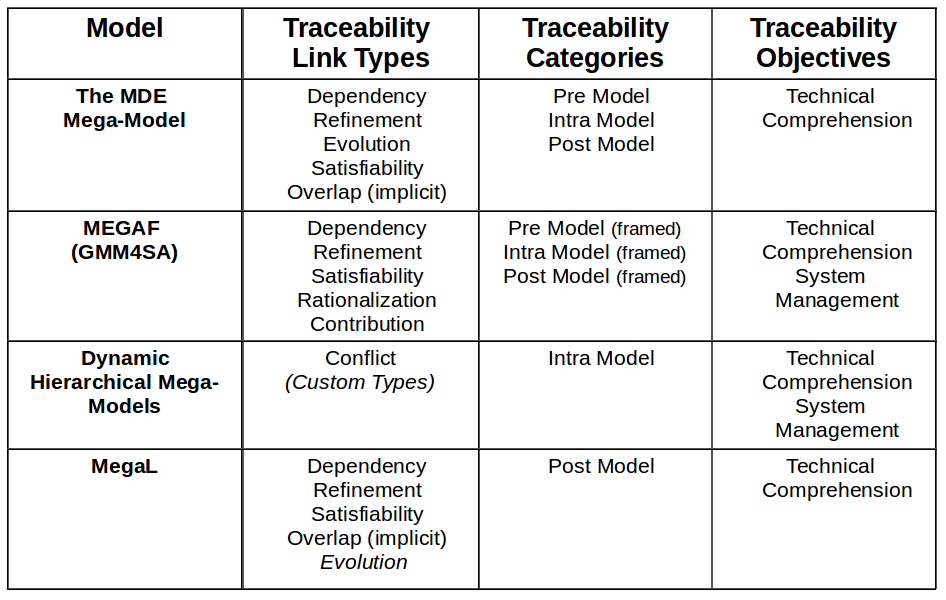
\includegraphics[width=0.7\textwidth]{ComparisonMatrix.png}
\caption{Comparison Result of selected MDE Mega-Models }
\label{fig:Comparison-Result-of-selected-MDE-Mega-Models}
\end{figure}

Figure \ref{fig:Comparison-Result-of-selected-MDE-Mega-Models} shows the result of our comparison.
It shows that the rather academical approaches, MegaL and the MDE-Mega-Model, are more interested in the technical aspectes of MDE.
Therefore their main traceability objective seems to be \textbf{Technical Comprehension} and only structural traceability links can be found (\textbf{Refinement, Dependency, Evolution, Overlap and Satisfiability}). 
In contrast to that, the approaches with enterprise tool support in mind, MEGAF and DHMM, enable traceability, which can provide additional information (\textbf{Contribution, Rationalization and Conflict}).
Moreover, they seem to also aim to support \textbf{System Management} as traceability objective.

The traceability categories according to Paige et al. seem to be a rather poor characteristic for comparison for mega-models.
But that is  not because of the categories itself than it is because of the varying abstraction levels of different mega-models.
For instance architecture frameworks formalize perspective.
Such perspective could be applied throughout the all categories for all model granularities.
That is why we annotated the categories in the result matrix with \textit{framed}.
Event the theoretical approaches (MegaL) could be extended to be used throughout the whole development process, although this is not always intended.
\newline
\newline
Future work on this topic could include:
\begin{itemize}

\item
the work on a more suitable categorization for traceability in general

\item
the study of traceability links, which exist only implicitly, such as the overlap link in the MDE-Mega-Model and MegaL.

\end{itemize}


%============================================================

\begin{thebibliography}{1}

\bibitem{DHMM}
A. Seibel, S. Neumann, and H. Giese. Dynamic hierarchical mega models: com- prehensive traceability and its efficient maintenance. Software \& Systems Mod- eling, 9(4):493–528, 2010.

\bibitem{Aizenbud-Reshef}
Aizenbud-Reshef, N., Nolan, B.T., Rubin, J., Shaham-Gafni, Y.:
Model traceability. IBM Syst. J. 45(3), 515–526 (2006)


\bibitem{GotelFinkelstein}
Gotel, O.C.Z., Finkelstein, A.C.W.: An analysis of the require-
ments traceability problem. In: 1st IEEE International Require-
ments Engineering Conference (RE’94) Proceedings, pp. 94–101.
IEEE Computer Society, New York (1994)

\bibitem{IEEEGlossary}
IEEE: IEEE Standard Glossary of Software Engineering Terminology, IEEE Std 610.12-1990

\bibitem{ISO/IEC42010}
ISO. ISO/IEC CD1 42010, Systems and software engineering
— Architecture description (draft), January 2010.

\bibitem{TowardsAMegamodel}
J.-M. Favre and T. NGuyen. Towards a Megamodel to Model Software Evolution through Transformations. ENTCS, 127(3), 2004. Proc. of the SETra Workshop.

\bibitem{MEGAL1}
Jean-Marie Favre, Ralf Lämmel, and Andrei Varanovich. Modeling the Linguistic Architecture of Software Products.

\bibitem{ScopedTraceability}
Lago, P., Muccini, H., van Vilet, H.: A scoped approacht to traceability management. J. Syst. Stoftw. 82(1), 168-182 (2009)

\bibitem{MEGAF}
R. Hilliard, I. Malavolta, H. Muccini, and P. Pelliccione. Realizing Architecture Frameworks Through Megamodelling Techniques. In Proc. of ASE’10, pages 305–308. ACM, 2010.

\bibitem{MEGAL2}
Ralf Lämmel and Andrei Varanovich. Interpretation of Linguistic Architectur. Unpublished, 2014

\bibitem{RameshEdwards}
Ramesh, B., Edwards, M.: Issues in the development of a require-
ments traceability model. In: Proceedings of the IEEE Interna-
tional Symposium on Requirements Engineering, pp. 256–259.
IEEE Computer Society, New York (1993)

\bibitem{PaigeEtAl}
Paige, R.F., Olsen, G.K., Kolovos, D.S., Zschaler, S., Power, C.:
Building model-driven engineering traceability classifications. In:
ECMDA Traceability Workshop (ECMDA-TW) 2008 Proceed-
ings, pp. 49–58. Sintef, Trondheim (2008). ISBN 978-82-14-
04396-9

\bibitem{Pinheiro}
Pinheiro, F.A.C.: Requirements traceability. In: Sampaio do Prado
Leite, J.C., Doorn, J.H. (eds.) Perspectives on Software Require-
ments, pp. 93–113. Springer, Berlin (2003)


\bibitem{TraceabilitySurvey}
S. Winkler and J. von Pilgrim. A survey of traceability in requirements engineer- ing and model-driven development. Software and System Modeling, 9(4):529– 565, 2010. 

\bibitem{OED}
Simpson, J., Weiner, E. (eds.): Oxford English Dictionary, vol. 18,
2nd edn. Clarendon Press, Oxford (1989). ISBN 978-0-198-
61186-8

\bibitem{SpanoudakisAndZisman}
Spanoudakis, G., Zisman, A. Software traceability: a roadmap. In:
Chang, S.K. (ed.) Handbook of Software Engineering and Knowl-
edge Engineering, vol. 3—Recent Advances, pp. 395–428. World
Scientific, Singapore (2005). ISBN 978-9-8125-6273-9

\bibitem{MegaRuntime}
Thomas Vogel, Andreas Seibel, and Holger Giese. The Role of Models and Megamodels at Runtime.


\end{thebibliography}

\end{document}